\chapter{Eksperymenty dla licencji Duolingo Super}
\label{chap:experiments}

\section{Środowisko i metodologia}

Eksperymenty wykonano na komputerze z procesorem Intel Core i5-14600KF (12 rdzeni, taktowanie 3,49~GHz) oraz 16~GB pamięci RAM. System operacyjny stanowił Ubuntu~24.04~LTS uruchomiony w środowisku WSL2. Implementacja algorytmów powstała w języku Python~3.13; wykorzystano biblioteki NumPy, NetworkX, a także PuLP jako interfejs do solverów ILP. Każdy pomiar obejmował wyłącznie czas obliczeń, pomijając koszt przygotowania instancji oraz operacje wejścia/wyjścia.

Analiza objęła dwa zestawy danych: (i) syntetyczne grafy losowe, bezskalowe oraz małoświatowe o liczebności od 50 do 450 wierzchołków, (ii) grafy ego z serwisu Facebook o liczebności od 53 do 1035 wierzchołków. Dla każdej instancji uruchamiano wszystkie algorytmy z limitem czasu wynoszącym 60~s. Przekroczenie limitu oznaczano jako \texttt{timeout} i wyłączano z dalszych obliczeń. Łącznie odnotowano 10 timeoutów dla \textbf{Algorytmu mrówkowego} oraz \textbf{Solvera~ILP} na grafach syntetycznych, a także odpowiednio 8, 18 i 6 przypadków dla \textbf{Algorytmu mrówkowego}, \textbf{Solvera~ILP} oraz \textbf{Przeszukiwania tabu} na grafach rzeczywistych. Wszystkie pozostałe uruchomienia zakończyły się sukcesem.

W przypadku grafów syntetycznych dla każdego rozmiaru generowano trzy niezależne instancje, a następnie wykonywano po dwa uruchomienia algorytmów na każdej z nich. Analiza sieci ego Facebooka obejmowała po jednym grafie na rozmiar oraz dwa powtórzenia dla każdej pary (graf, algorytm), co pozwoliło oszacować zmienność wyników przy zachowaniu rozsądnego budżetu obliczeniowego.

W każdej próbie zapisano całkowity koszt licencji, czas wykonania oraz koszt w przeliczeniu na wierzchołek. Wyniki agregowano przez medianę oraz średnią. Spójność różnic między algorytmami oceniono przy użyciu testów Friedmana oraz następujących po nich porównań post-hoc metodą Nemenyi'ego. Na syntetycznym benchmarku otrzymano statystyki $\chi^2_F = 577{,}93$ dla czasu oraz $\chi^2_F = 518{,}01$ dla kosztu na węzeł ($p < 10^{-100}$ w obu przypadkach), co uzasadnia szczegółowe porównania par algorytmów.

\section{Duolingo Super na grafach syntetycznych}

\subsection{Statystyki zbiorcze}

Tabela~\ref{tab:duo-synth-summary} zestawia mediany i średnie wartości kosztu oraz czasu dla licencji Duolingo Super. \textbf{Solver~ILP} pozostaje najlepszym punktem odniesienia jakościowego (mediana kosztu 42,45), lecz przydaje się jedynie dla mniejszych instancji. Posiada tyle samo timeoutów co \textbf{Algorytm mrówkowy}. Wśród metaheurystyk najniższy koszt osiąga właśnie \textbf{Algorytm mrówkowy} (0,445 kosztu na węzeł), natomiast \textbf{Przeszukiwanie tabu} zapewnia najlepszy kompromis kosztu i czasu w grupie metod przybliżonych. \textbf{Algorytm zachłanny} i \textbf{Algorytm losowy} działają prawie natychmiast, ale tylko pierwszy z nich zachowuje akceptowalny koszt (0,493), podczas gdy losowy baseline pozostaje wyraźnie gorszy jakościowo.

\begin{table}[H]
  \centering
  \caption{Statystyki kosztu i czasu dla licencji Duolingo Super na grafach syntetycznych.}
  \label{tab:duo-synth-summary}
  \begin{tabular}{lrrrr}
    \toprule
    \textbf{Algorytm}     & \textbf{Mediana kosztu} & \textbf{Średni koszt} & \textbf{Mediana czasu [s]} & \textbf{Średni czas [s]} \\
    \midrule
    Solver ILP            & 42.45                   & 73.83                 & 0.792                      & 2.492                    \\
    Algorytm mrówkowy     & 62.50                   & 83.58                 & 1.978                      & 5.124                    \\
    Przeszukiwanie tabu   & 67.30                   & 117.80                & 1.423                      & 3.298                    \\
    Algorytm genetyczny   & 69.30                   & 118.36                & 0.525                      & 1.222                    \\
    Wyżarzanie symulowane & 72.30                   & 120.90                & 0.404                      & 0.975                    \\
    Zbiór dominujący      & 71.38                   & 119.97                & 0.003                      & 0.017                    \\
    Algorytm zachłanny    & 72.30                   & 121.94                & 0.001                      & 0.001                    \\
    Algorytm losowy       & 108.92                  & 179.90                & 0.001                      & 0.001                    \\
    \bottomrule
  \end{tabular}
\end{table}


\subsection{Wnioski z analizy kosztów i czasów}

Rysunki~\ref{fig:duo-synth-cost-random}--\ref{fig:duo-synth-cost-small-world} pokazują, że algorytmy dla licencji Duolingo Super osiągają wyniki porównywalne z solverem ILP w przypadku grafów losowych i małoświatowych. Natomiast w przypadku grafów bezskalowych wyniki są zauważalnie gorsze.


\begin{figure}[H]
  \centering
  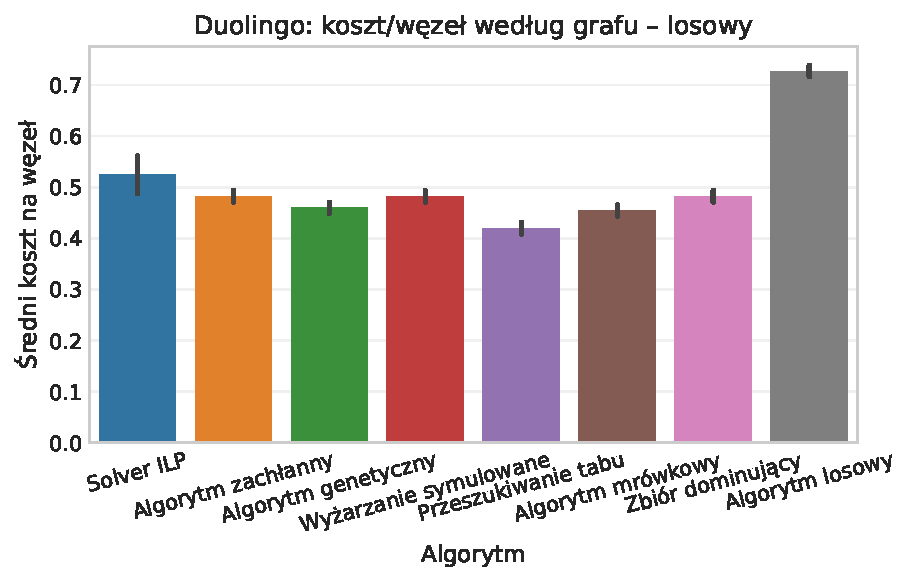
\includegraphics[width=0.65\linewidth]{assets/figures/benchmark/synthetic/duolingo_cost_per_node_by_graph_random.pdf}
  \caption{Koszt na węzeł w zależności od struktury grafu losowej.}
  \label{fig:duo-synth-cost-random}
\end{figure}

\begin{figure}[H]
  \centering
  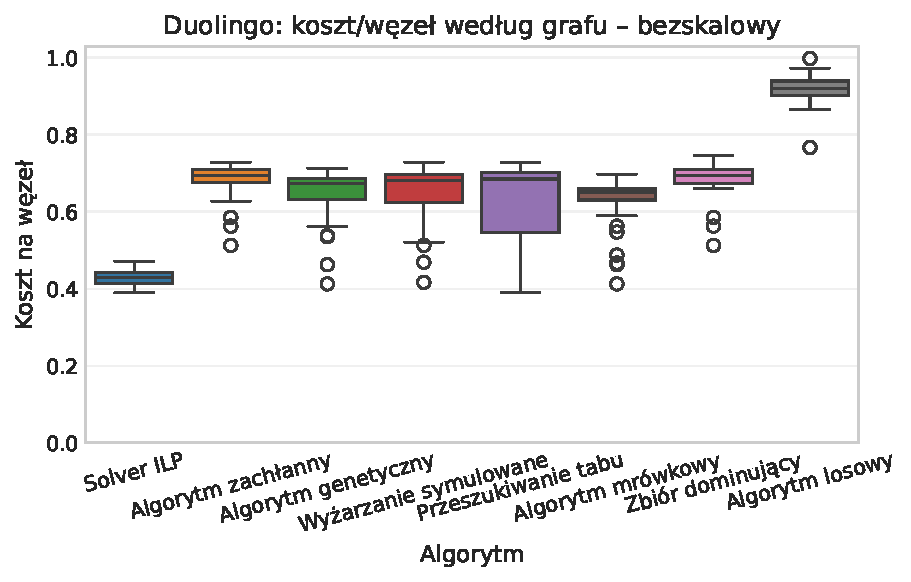
\includegraphics[width=0.65\linewidth]{assets/figures/benchmark/synthetic/duolingo_cost_per_node_by_graph_scale_free.pdf}
  \caption{Koszt na węzeł w zależności od struktury grafu bezskalowej.}
  \label{fig:duo-synth-cost-scale-free}
\end{figure}

\begin{figure}[H]
  \centering
  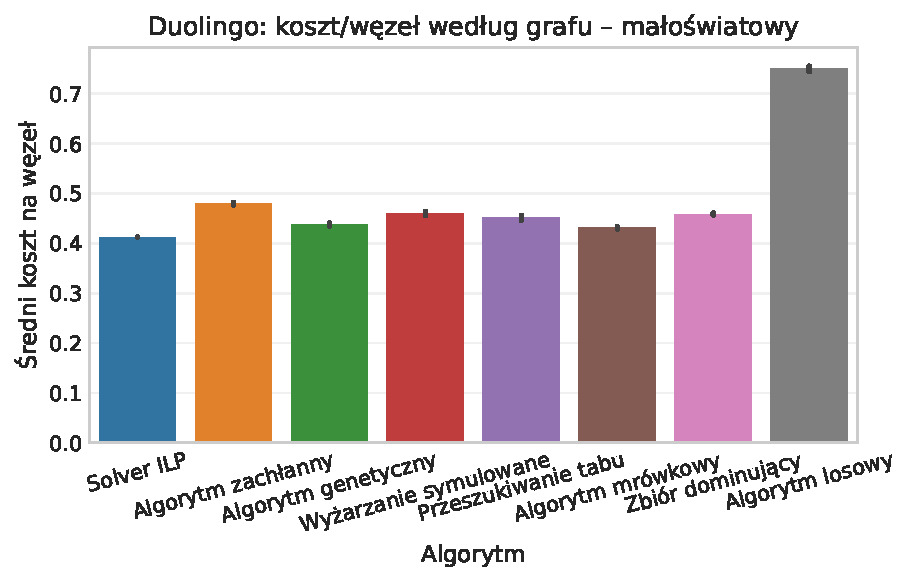
\includegraphics[width=0.65\linewidth]{assets/figures/benchmark/synthetic/duolingo_cost_per_node_by_graph_small_world.pdf}
  \caption{Koszt na węzeł w zależności od struktury grafu małoświatowej.}
  \label{fig:duo-synth-cost-small-world}
\end{figure}

Podobne obserwacje dotyczą czasów wykonania, jak ilustrują rysunki~\ref{fig:duo-synth-time-random}--\ref{fig:duo-synth-time-small-world}. Średnie czasy działania algorytmów są najniższe dla grafów małoświatowych i losowych, natomiast dla grafów bezskalowych są wyraźnie wyższe. Tabela~\ref{tab:duo-synth-summary-times} podsumowuje mediany czasów i kosztów na węzeł dla różnych typów grafów.



\begin{figure}[H]
  \centering
  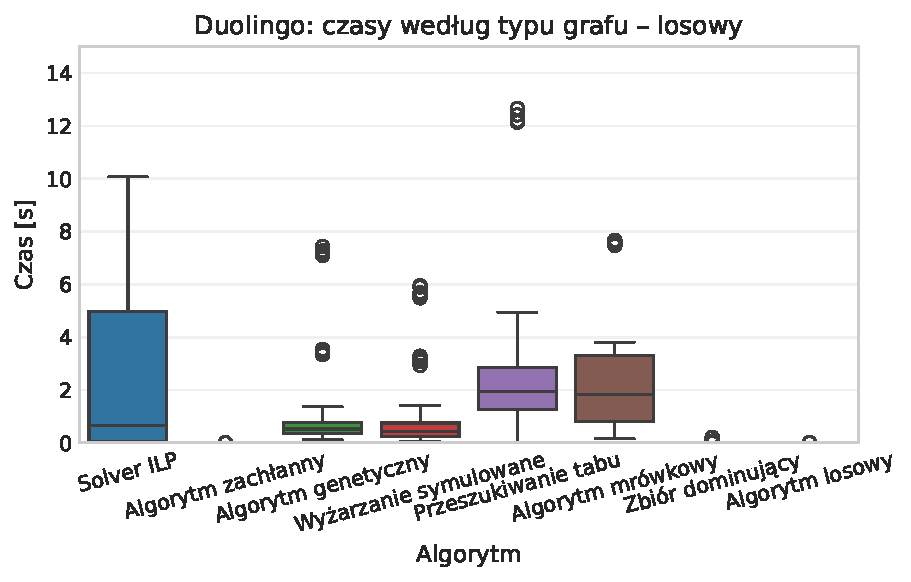
\includegraphics[width=0.65\linewidth]{assets/figures/benchmark/synthetic/duolingo_time_by_graph_random.pdf}
  \caption{Czas wykonania w zależności od struktury grafu losowej.}
  \label{fig:duo-synth-time-random}
\end{figure}

\begin{figure}[H]
  \centering
  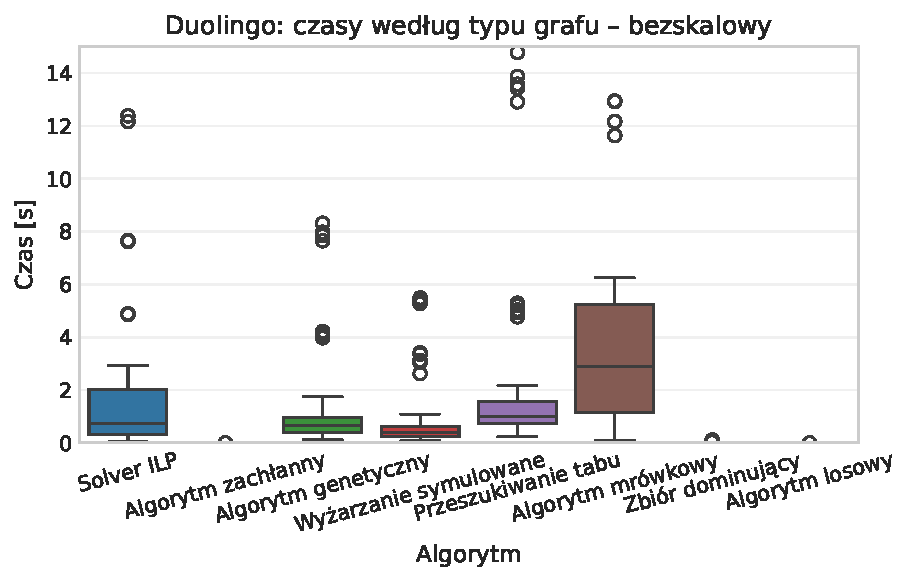
\includegraphics[width=0.65\linewidth]{assets/figures/benchmark/synthetic/duolingo_time_by_graph_scale_free.pdf}
  \caption{Czas wykonania w zależności od struktury grafu bezskalowej.}
  \label{fig:duo-synth-time-scale-free}
\end{figure}

\begin{figure}[H]
  \centering
  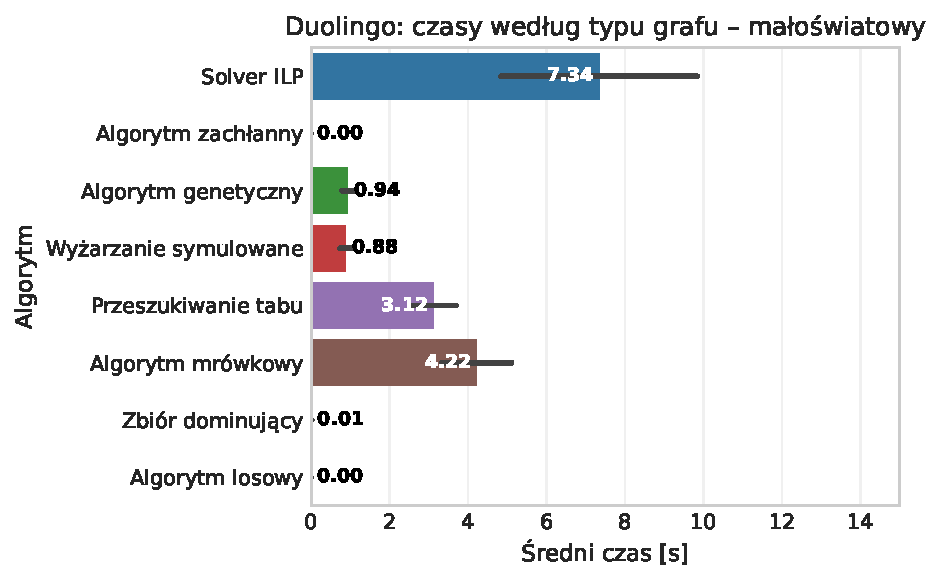
\includegraphics[width=0.65\linewidth]{assets/figures/benchmark/synthetic/duolingo_time_by_graph_small_world.pdf}
  \caption{Czas wykonania w zależności od struktury grafu małoświatowej.}
  \label{fig:duo-synth-time-small-world}
\end{figure}


\begin{table}[H]
  \centering
  \caption{Mediany czasów i kosztów na węzeł dla różnych typów grafów (Duolingo Super i dominowanie rzymskie).}
  \label{tab:duo-synth-summary-times}
  \begin{tabular}{lcccc}
    \toprule
    \textbf{Licencja}    & \textbf{Typ grafu} & \textbf{Med. czas [s]} & \textbf{Med. koszt/węzeł} \\
    \midrule
    Duolingo Super       & Bezskalowy         & 0.315                  & 0.680                     \\
    Duolingo Super       & Losowy             & 0.207                  & 0.453                     \\
    Duolingo Super       & Małoświatowy       & 0.203                  & 0.466                     \\
    Dominowanie rzymskie & Bezskalowy         & 0.211                  & 0.460                     \\
    Dominowanie rzymskie & Losowy             & 0.215                  & 0.300                     \\
    Dominowanie rzymskie & Małoświatowy       & 0.254                  & 0.375                     \\
    \bottomrule
  \end{tabular}
\end{table}

Z powyższych danych wynika, że struktura grafu ma istotny wpływ zarówno na koszty, jak i na czasy działania algorytmów. Licencja Duolingo Super radzi sobie najgorzej w przypadku grafów bezskalowych. Z kolei licencja dominowania rzymskiego osiąga najgorsze wyniki dla grafów małoświatowych, podczas gdy w przypadku grafów bezskalowych wypada najlepiej.

\section{Duolingo Super na grafach rzeczywistych}

W analizie grafów ego z serwisu Facebook pominięto obserwacje, w których solver ILP nie zakończył pracy przed limitem czasu (18 przypadków). Dodatkowo odnotowano 8 timeoutów algorytmu mrówkowego i 6 przypadków w przeszukiwaniu tabu; pozostałe uruchomienia zakończyły się sukcesem.

\begin{table}[H]
  \centering
  \caption{Statystyki kosztu i czasu dla licencji Duolingo Super na grafach rzeczywistych.}
  \label{tab:duo-real-alg}
  \begin{tabular}{lrrrrr}
    \toprule
    \textbf{Algorytm}     & \textbf{Średni koszt} & \textbf{Śr. koszt/węzeł} & \textbf{Śr. czas [s]} \\
    \midrule
    Algorytm mrówkowy     & 83.58                 & 0.506                    & 5.124                 \\
    Algorytm genetyczny   & 118.36                & 0.515                    & 1.222                 \\
    Przeszukiwanie tabu   & 117.80                & 0.500                    & 3.298                 \\
    Zbiór dominujący      & 119.97                & 0.542                    & 0.017                 \\
    Wyżarzanie symulowane & 120.90                & 0.531                    & 0.975                 \\
    Algorytm zachłanny    & 121.94                & 0.548                    & 0.001                 \\
    Algorytm losowy       & 179.90                & 0.799                    & 0.001                 \\
    \bottomrule
  \end{tabular}
\end{table}
Tab.~\ref{tab:duo-real-alg} pokazuje, że zarówno przeszukiwanie tabu, jak i algorytm mrówkowy zachowują przewagę kosztową nad heurystykami losowymi i zachłannymi, choć okupują ją dłuższym czasem działania.

\subsection{Skalowanie i jakość}

Rysunek~\ref{fig:duo-real-size} pokazuje, że wraz ze wzrostem liczby wierzchołków koszt na węzeł rośnie umiarkowanie, przy czym przeszukiwanie tabu utrzymuje najniższe wartości, a algorytm mrówkowy plasuje się tuż za nim. Czasy działania wszystkich metod mieszczą się w przedziale do kilku sekund i rosną łagodnie wraz z rozmiarem grafu; algorytm zachłanny nadal pozostaje niemal natychmiastowy i stanowi dobry punkt startowy dla metaheurystyk. Dodatkowo tab.~\ref{tab:duo-real-size-table} zbiera średnie wartości (TabuSearch) dla kolejnych rozmiarów sieci ego i pokazuje, że koszt na węzeł utrzymuje się w przedziale 1{,}8--2{,}5 przy czasie rosnącym od ułamka sekundy do około 5{,}5~s dla największych grafów.

\begin{figure}[H]
  \centering
  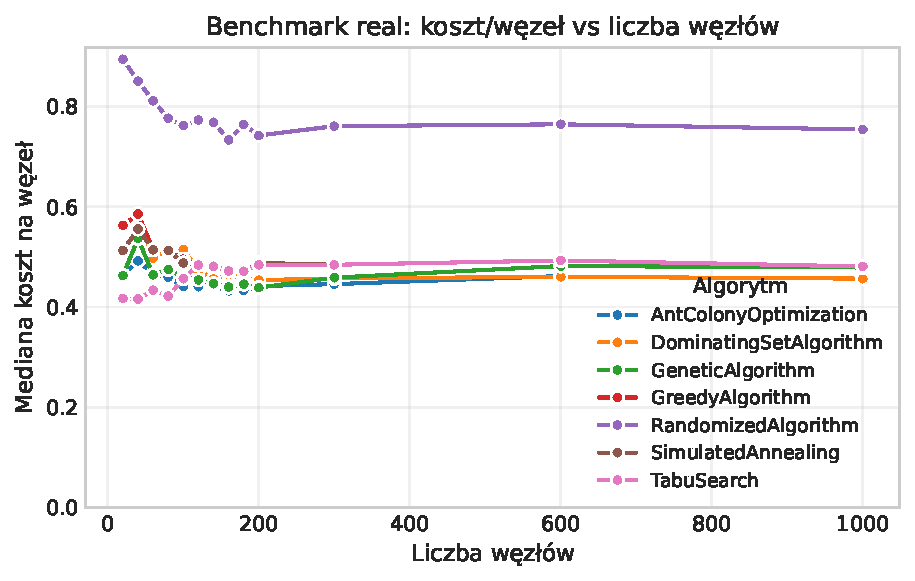
\includegraphics[width=0.48\linewidth]{assets/figures/benchmark/real/cost_per_node_vs_nodes.pdf}
  \hfill
  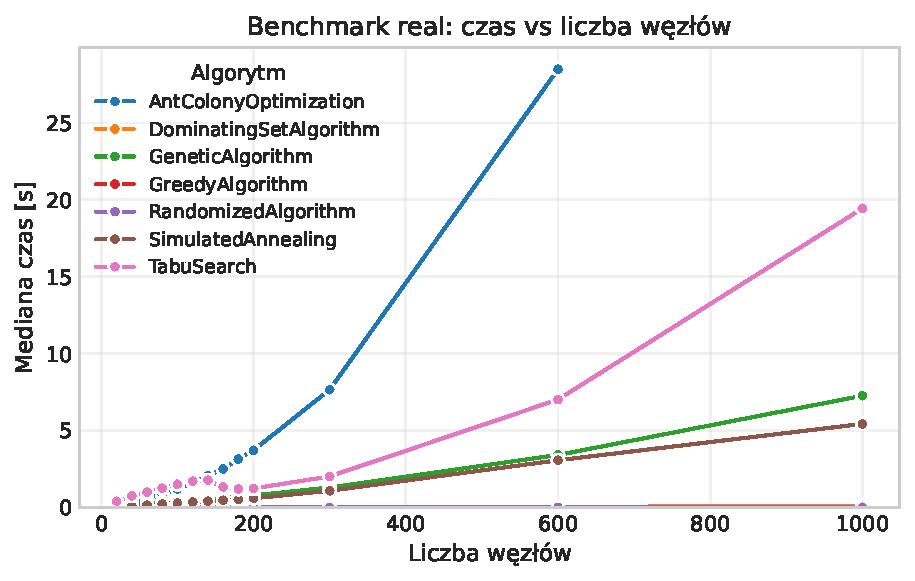
\includegraphics[width=0.48\linewidth]{assets/figures/benchmark/real/time_vs_nodes.pdf}
  \caption{Koszt na węzeł i czas wykonania licencji Duolingo Super w funkcji liczby wierzchołków (grafy ego Facebook).}
  \label{fig:duo-real-size}
\end{figure}

\begin{table}[H]
  \centering
  \caption{Średni koszt na węzeł i czas (przeszukiwanie tabu) względem liczby wierzchołków w sieciach ego Facebook.}
  \label{tab:duo-real-size-table}
  \begin{tabular}{lrr}
    \toprule
    extbf{Liczba wierzchołków} & \textbf{Śr. koszt/węzeł} & \textbf{Śr. czas [s]} \\
    \midrule
    53                         & 2.061                    & 0.195                 \\
    62                         & 1.800                    & 0.205                 \\
    151                        & 1.773                    & 0.511                 \\
    169                        & 1.836                    & 0.597                 \\
    225                        & 1.942                    & 0.833                 \\
    334                        & 2.459                    & 1.528                 \\
    535                        & 2.427                    & 2.450                 \\
    748                        & 2.034                    & 3.842                 \\
    787                        & 2.205                    & 3.775                 \\
    1035                       & 2.168                    & 5.485                 \\
    \bottomrule
  \end{tabular}
\end{table}


\section{Porównanie z dominowaniem rzymskim}

Porównania z dominowaniem rzymskim ograniczono do wspólnych instancji i algorytmów. Rysunki~\ref{fig:duo-roman-cost}--\ref{fig:duo-roman-license} zestawiają różnice w kosztach, czasach i strukturze licencji, a tabela~\ref{tab:duo-roman-graph} gromadzi mediany według typu grafu syntetycznego.

\begin{table}[H]
  \centering
  \caption{Mediany czasu i kosztu na węzeł według typu grafu (wspólne instancje).}
  \label{tab:duo-roman-graph}
  \begin{tabular}{lcccc}
    \toprule
    \multirow{2}{*}{\textbf{Typ grafu}} & \multicolumn{2}{c}{\textbf{Duolingo Super}} & \multicolumn{2}{c}{\textbf{Dominowanie rzymskie}}                                            \\
                                        & \textbf{Czas [s]}                           & \textbf{Koszt/węzeł}                              & \textbf{Czas [s]} & \textbf{Koszt/węzeł} \\
    \midrule
    Losowy                              & 0.205                                       & 0.453                                             & 0.201             & 0.288                \\
    Bezskalowy                          & 0.222                                       & 0.686                                             & 0.162             & 0.478                \\
    Małoświatowy                        & 0.193                                       & 0.467                                             & 0.173             & 0.387                \\
    \bottomrule
  \end{tabular}
\end{table}

Dominowanie rzymskie zapewnia niższy koszt na węzeł we wszystkich porównywanych rodzinach grafów. Największa różnica dotyczy struktur losowych, gdzie przewaga wynosi ok.~0,16 punktu (35\%). W sieciach bezskalowych rozpiętość maleje do 0,21, natomiast w małoświatowych do 0,08. Czasy wykonania pozostają porównywalne, przy lekkiej przewadze dominowania rzymskiego (różnica 10--25~ms). Rysunek~\ref{fig:duo-roman-cost} ilustruje te obserwacje dla pełnego rozkładu, a rysunek~\ref{fig:duo-roman-time} prezentuje analogiczne dane czasowe. Warto jednak zauważyć, że wyższe koszty na węzeł w przypadku Duolingo Super wynikają z większego udziału licencji grupowych, które obejmują średnio 2,1 użytkownika i są droższe od licencji indywidualnych. To właśnie ten czynnik znacząco wpływa na różnice w kosztach między obiema konfiguracjami.

\begin{figure}[H]
  \centering
  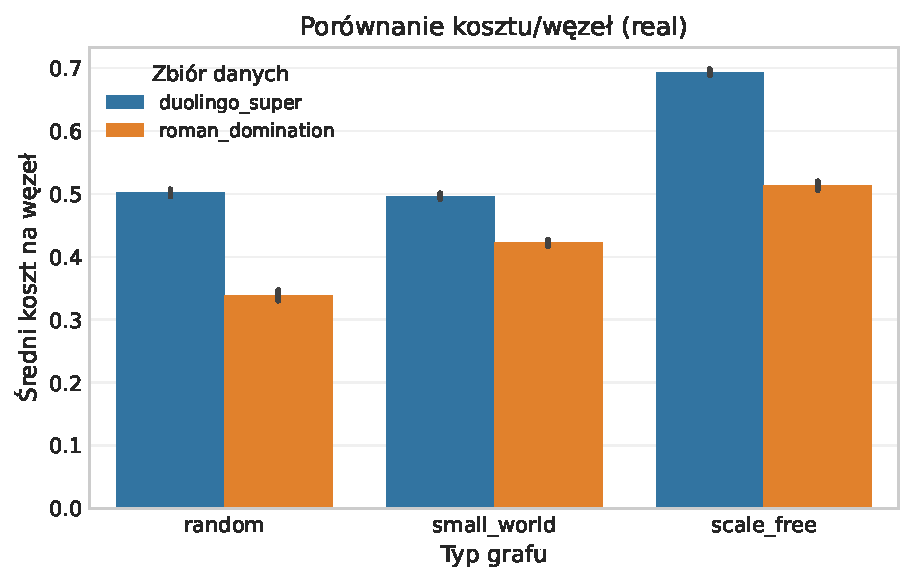
\includegraphics[width=0.6\linewidth]{assets/figures/benchmark/real/duo_vs_roman_cost_per_node_by_graph.pdf}
  \caption{Koszt na węzeł według typu grafu: porównanie licencji Duolingo Super i dominowania rzymskiego.}
  \label{fig:duo-roman-cost}
\end{figure}

\begin{figure}[H]
  \centering
  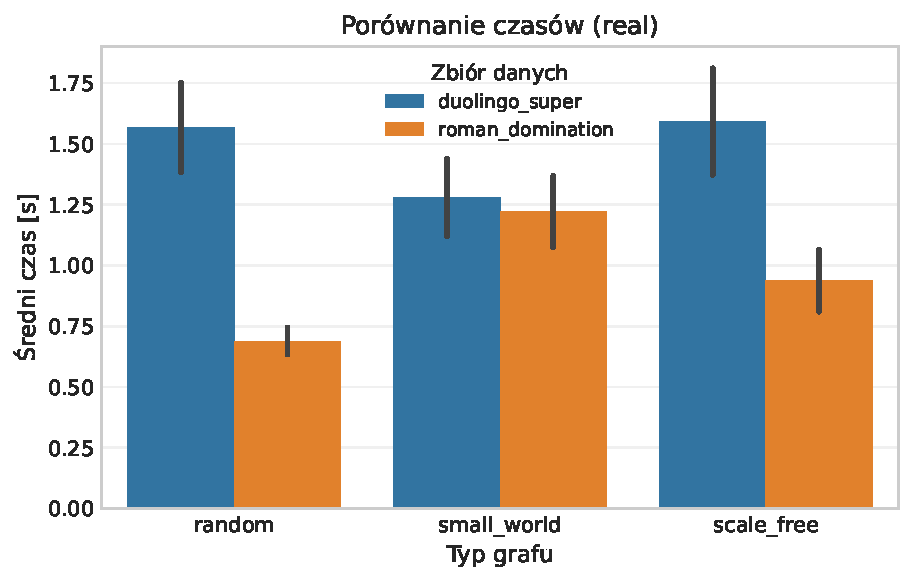
\includegraphics[width=0.6\linewidth]{assets/figures/benchmark/real/duo_vs_roman_time_by_graph.pdf}
  \caption{Czas wykonania według typu grafu: porównanie licencji Duolingo Super i dominowania rzymskiego.}
  \label{fig:duo-roman-time}
\end{figure}

Rysunek~\ref{fig:duo-roman-license} pokazuje, że dominowanie rzymskie charakteryzuje się wyższym stosunkiem licencji grupowych do indywidualnych w porównaniu do Duolingo Super. W przypadku dominowania rzymskiego stosunek ten wynosi około 1,15:1, podczas gdy dla Duolingo Super jest to około 0,88:1.

Różnica ta wynika z faktu, że dominowanie rzymskie nie posiada ograniczenia maksymalnej pojemności grupy licencyjnej. W przypadku Duolingo Super, gdy grupa osiąga maksymalną pojemność, dodatkowi użytkownicy, którzy mogliby do niej należeć, są zmuszeni do zakupu licencji indywidualnych. W pełnym zbiorze danych, obejmującym trzy typy grafów syntetycznych, zaobserwowano 137690 licencji w Duolingo Super, z czego 73176 (53,15\%) to licencje indywidualne. W przypadku dominowania rzymskiego, dzięki braku ograniczeń pojemności grup, liczba licencji indywidualnych jest proporcjonalnie niższa.

\begin{figure}[H]
  \centering
  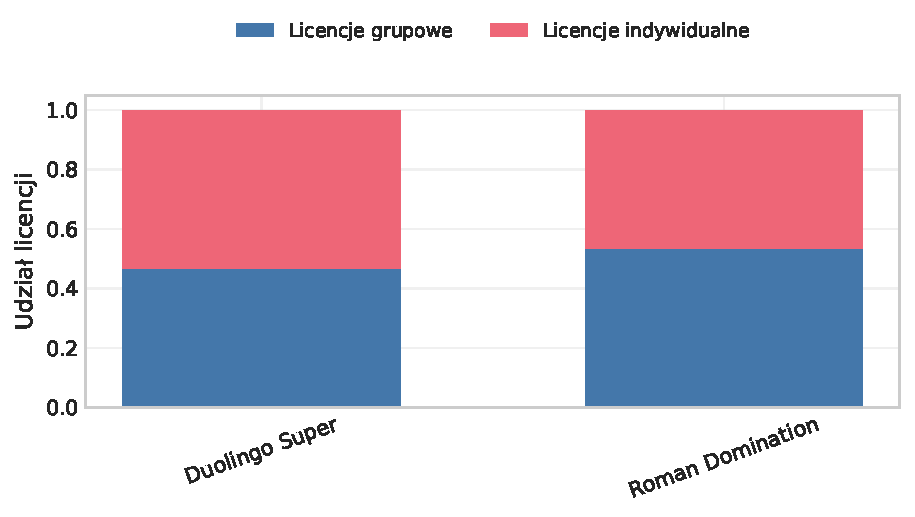
\includegraphics[width=0.6\linewidth]{assets/figures/benchmark/synthetic/license_mix_duo_vs_roman.pdf}
  \caption{Struktura wykorzystania licencji: porównanie licencji Duolingo Super i dominowania rzymskiego.}
  \label{fig:duo-roman-license}
\end{figure}

\section{Wnioski}

Analiza potwierdza dużą stabilność wyników Duolingo Super: metaheurystyki utrzymują przewagę jakości nad prostymi heurystykami niezależnie od rozmiaru i struktury grafu, a \textbf{Algorytm mrówkowy} oraz \textbf{Przeszukiwanie tabu} stanowią najbardziej konkurencyjną parę. Równocześnie dominowanie rzymskie pozostaje trudne do pobicia pod względem kosztu na węzeł, głównie dzięki większemu wykorzystaniu licencji grupowych i niższemu mnożnikowi kosztów jednostkowych.
